\documentclass[9pt,a4paper]{acmproc}
\usepackage[utf8]{inputenc}
\usepackage{amsmath}
\usepackage{amsfonts}
\usepackage{amssymb}
\usepackage{graphicx}
\usepackage[english]{babel}
\usepackage[utf8]{inputenc}
\usepackage{amsmath}
\usepackage{cite}
\usepackage{afterpage}


\graphicspath{}

\author{
\texttt{Andreas Nordberg}\\
\texttt{andno793@student.liu.se}
  \and
  \texttt{Jonathan Sjölund}\\
  \texttt{jonsj507@student.liu.se}
}

\begin{document}


\title{%
	Geo-based media player \\
	\large An interactive interface for geo-based video streaming}
\maketitle

%%Ta bort två sidor
%\cleardoublepage

\pagenumbering{arabic}
%\setcounter{page}{3}

\begin{abstract}
Being able to interact with a video stream can be both fun, educational and provide help during disaster situations however, to achieve the best user experience, the interaction must be seamless. Creating a media player that can allow users to view a video stream from different geographical positions is a challenge that is tackled in this paper. This paper describes the material and methods used to accomplish this kind of media player. And it explains how to achieve a seemingly good and, to higher extent, enjoyable video streaming experience. An algorithm is developed for placing each object on a geographical based map automatically. The objects are placed to ensure that relativity compared to the real world is kept. A proof-of-concept is shown of a media player that enables a user to see an overview over a geographical streaming location. By seeing each streams relative location to the point-of-interest the users are able to click on that stream and switch to it, however not in a seamless way. This project shows the command-and-control center envisioned but without a seamless switch. Instead the work done and the code provided will allow for prefetching to be added in future work in an easy way.

\end{abstract}

\begin{keywords}
HTTP Adaptive Streaming (HAS), OSMF video player, Interactive video streaming, Geographical based streaming (GBS), Command-and-Control Center
\end{keywords}

\section{Introduction} 

Streaming has evolved and become more popular over last couple of years. Thousands upon thousands of different streams are being watched every day\footnote{Twitch statistics https://stats.twitchapps.com/, Fetched: 2016-04-01}, thus the demand for better and more ways to stream are longed for. If we could stream videos in different ways we can create a more interesting streaming environment, this can provide both better entertainment but also a better way to potentially improve observation in science and other areas more reliably. If a stream can provide the possibility for watching a video from different angles it can give people the option to observe and also enjoy something from different perspectives. This project focuses on accomplishing that, by creating a geo-based video player that uses HTTP-adaptive streaming (HAS) that can allow people to view a video from different angles and change between them seamlessly without any buffering delay or stuttering. By looking at an existing video streaming player and improve it to accomplish this task we show that it is something worth implementing in already existing media players.

In this project we design and develop a geo-based command-and-control video streaming player using geo-tags. In practice this means that a service in which you can choose between a set of recording streams of the same event, for example, but slightly different locations and angles. This would be a useful feature to have in any larger event where you would want to show the same scene from different locations and angles. The interface will be useful for both event-organizers that hire staff to make several different recordings of the same scene for simultaneous viewing, but could also be used by the public who volunteer to record the event live. One major thing that this also could be used for is during a disaster event or something similar. By helping the police, medical and the emergency service by allowing them to view a disaster scenario from angles that can help them in communication. To be able to see and interactive with how the situation is seen from different angles to give a better understanding of what needs to be done.

\subsection{Boundaries}
The application we provide is only going to be a proof-of-concept which means that we will only focus on the functionality of the video player. Factors like a pretty interface and usability on broader spectrum will be neglected. We will focus on making the application work for only one user to verify the functionality we want to accomplish. The number of video streams that we will be able to switch between will,for the purpose of testing, be limited to a few, but then expanded upon to support any reasonable number of streams. This is because we firstly want to make sure that it is possible to switch between video streams and not that it can be done over large numbers. The reason for this is that pre-buffering many videos can be difficult to accomplish with a large number of video streams. As long as we provide a way to do it the solution can be expanded upon.


\section{Background and Related Work}
To be able to grasp the concept of how HTTP-adaptive streaming (HAS) and geo-based streaming (GBS) works we first present background on HAS and GBS in order to further strengthen our methodology and the interpretation of our result. Since we are using HAS and GBS when programming our interface there is a need to study existing works and articles. By using that knowledge it becomes possible to implement a new upgraded media player that is adapted to streaming from different geographical positions.

There are many related works to our work. Many of these works are focusing on branching videos in media players, which describes ways to allow for users to seamlessly switch between videos without quality degradation or interruptions \cite{qualbranch, hasmultipath,scalableOnDemand}. Zhao et al. \cite{scalableOnDemand} propose protocols that enables the possibility of scaleable on-demand content with minimal server load and developing a way that limits the lower bound bandwidth requirement using multicast \cite{scalableOnDemand}. Other works talks about policies for providing a good way of prefetching several videos in different ways, providing means of allowing prefetching and instantaneous playback without playback quality degradation. The work studies the off-periods observed in HAS-players to utilize it as effectively as possible \cite{bandawarePrefetch}.

There are also works that have looked at optimiziation of video quality by observing and controlling the playback buffer by in turn looking at the network capacity, providing an algorithm for optimizing the video quality without any unnecessary buffering \cite{bufferbased}.

\subsection{HTTP-based Adaptive Streaming}
Mobile users streaming media sometimes suffers from playback interruption when faced with a bad wireless connection. HTTP-adaptive streaming seeks to resolve this by dynamically changing the bitrate and therefore quality of the stream to make do with the connection that is available to the user. To ensure smooth transitions between these quality swaps HAS also tries to predict the swaps in advance using various methods depending on the HAS framework. There are many algorithms for these predictions, but a brief example would be to use previous logged connectivity history and future connectivity using geo-based methods to make predictions \cite{gtube}. Most HAS players uses weighted average of past download time/rates in order to estimate download rate of available bandwidth \cite{qualbranch}. With these HAS predictions, a stream quality fitting the user’s network quality can be buffered \cite{gtube}.

With HAS-adaptive streaming it is needed for us to prefetch data from several close-by streams (if not all, depending on number of them) and build up a small enough buffer that makes switching between different streams seamless. By looking at how HAS is used when implementing an interactive branched video we can say that parallel TCP connections is a must in-order to achieve this with a cost of wasting bandwidth and lower playback quality. This depends mainly on the number of videos that needs to be prefetched. Most HAS video players has a cap on the buffer size in order to avoid wasting bandwidth. Krishnamoorthi et al. \cite{qualbranch} use a customized HAS player that solves the problem of trade-off between quality and number of chunks downloaded. The playback chunks are stored in the playback buffer while the prefetched chunks are stored in a browser cache thus allowing those chunks to be retrieved quickly. This ensures that no playback interruption occurs for the user. The way they download the chunks are done in a round-robin way to ensure that a buffer workahead is built up enough for seamless playback in parallel TCP downloading. 

Downloading chunks in a round-robin way is how chunks will be downloaded in our media player. This way will be used together with the idea of prefetching in the downtime of a HAS-player. Most HAS-players has some kind of buffer treshold $T_{max}$ where downloading is interrupted when reached and will resume only when the minimum buffer $T_{min}$ is reached. This kind of behaviour can be called an \textit{on-off behaviour} which can lead to poor performance under conditions with competing traffic. It is common in several HAS-players like Netflix and Microsoft Smooth Streaming for example. Krishnamoorthi et al. \cite{bandawarePrefetch} provide policies and ideas that reduce the start-up time of videos by an order of magnitude and ensures the highest possible playback quality to be viewed. A way of improved channel utilization that allows for instantaneous playback of prefetched videos. They provide an HAS solution which we will take advantage of together with prefecthing nearby streams in a round-robin way. The solution allows for prefetching and buffer management in such a way that videos can be downloaded parallel and switched to instantaneous without interrupting the user experience. By using a novel system to utilize the unused bandwidth during off periods this allows for videos to simultaneously be prefetched while maintaining a fair bandwidth share. It also increases the playback quality in which a video is downloaded \cite{bandawarePrefetch}. This idea will be discussed further in section 2.2 when we describe our idea of downloading streams.

There can occur several problems in HAS players \cite{qualbranch}. Huang et al. \cite{streamrate} show that when a competing TCP flow starts a so called “downward spiral effect” occurs and the downgrade in throughput and playback rate becomes severe. This is caused by a timeout in the TCP congestion window, high packet loss in competing flows and when a client has a lower throughput the playback rate is lower due to smaller buffer segments which makes a video flow more susceptible to perceiving lower throughput and thus creating a spiral. A possible solution is to have larger segment size and by having an algorithm which is less conservative, meaning that requesting a video at lower rate than is perceived. This is something that we can keep in mind since quality can decrease drastically when having several videos buffering in parallel, though we will not have to buffer a full video at the same time but only chunks of a video while the main stream is being watched.

\subsection{Non-linear Streaming and Multipath}
Krishnamoorthi et al. \cite{hasmultipath} use this technique of storing prefetched chunks in a playback buffer simliar to [6]. Prefetching for different branches to allow seamless switching between videos, using the notion of multi-path nonlinear videos to stitch together videos using a novel buffer management and prefetching policy. This prefetching decreases the time it takes to switch between branches considerably and is something we will take advantage of since the code we use from \cite{qualbranch} are based on a similar policy \cite{hasmultipath}. If we look at what Zhao et al. \cite{scalableOnDemand} wrote they describe how choosing a correct branching point sufficiently ahead of time with an accuracy of 75 \% greatly reduces bandwidth requirements. Requesting nonlinear video content where chunks are downloaded parallel without causing jitter. This is something which is really important and efficient for users that would like the ability to switch between different videos on-demand. Selecting what type of chunks should be downloaded is hard to accomplish, atleast on a broader context when considering watching TV stream during TV broadcasting \cite{scalableOnDemand}.  Most of these works are mostly focused on branching videos which is simliar but not entierly simliar to what we will be doing \cite{qualbranch, hasmultipath,scalableOnDemand}. We will contribute more to the possibility of prefetching several videos parallel and then be able to switch to any of  them on-demand. However the ideas used when handling branching videos is something that will be used in our mediaplayer.

Figure \ref{fig:HAS1} and \ref{fig:HAS2} illustrate an example of a stream consisting of chunks being played, how these chunks are prefetched and stored and a swap between two streams.

\begin{figure}[!ht]
\begin{center}
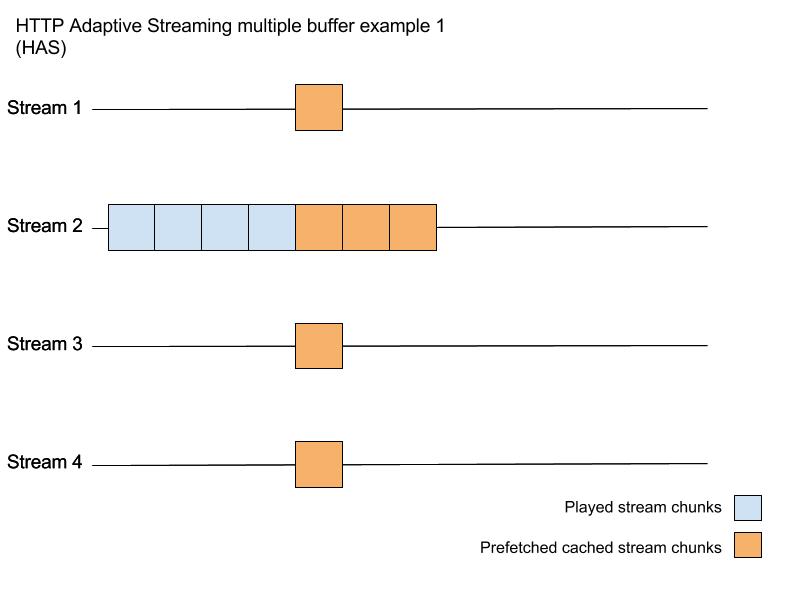
\includegraphics[scale=0.3]{HAS1.png}
\caption{HAS Parallell Stream Buffer 1}
\label{fig:HAS1}
\end{center}
\end{figure}

\begin{figure}[!ht]
\begin{center}
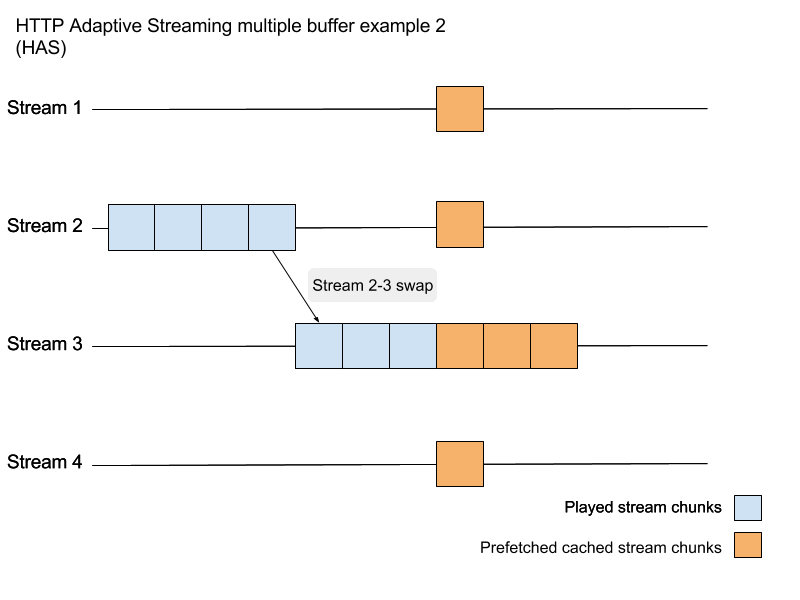
\includegraphics[scale=0.3]{HAS2.png}
\caption{HAS Parallell Stream Buffer 2}
\label{fig:HAS2}
\end{center}
\end{figure}



\subsection{Strobe Media Playback}

To display the stream in our application we will be using a media player called Strobe Media Playback (SMP), created with the Open Source Media Framework (OSMF) by Adobe Systems. The OSMF itself is build upon Adobe Flash Player, while becoming more outdated by day and discontinued by some, is widely used for media and other graphic applications and suffices to use for the proof-of-concept of our application. In practice this means that the media player is created using the tools that OSMF provides, compiled into a runnable flash file bytecode and run by Adobe Flash Player. 
OSMF supports a number of important features that will be used within our interface. Most importantly it enables the use of HAS with its HTTP streaming support and progressive downloading. It also enables the player to seamlessly switch between several media elements by using a composition of “nested serial elements”, which will be prominently used within our application.\cite{osmf}

\section{System Design}

To advance in this project we will mainly be programming, designing and developing the application. The programming language of choice will be Adobe ActionScript and the IDE Flash Builder, which is very similar to the IDE Eclipse. The functionality of the interface to be developed is multiple. We want the interface to accept incoming video streams tagged with a location and cardinal direction from expected sources. The video streams will have to be tagged with these geographical datas somehow, which is not a common included feature with most video recording softwares. Developing a separate recording application to create these kind of video streams, for the sake of this project, might be outside of our goal of limitations for this project. If it is, we will prove the functionality of our interface with fabricated video geo-tags. These streams will then be made to work with the custom OSMF player.  Under-the-hood features will include HAS to ensure a smooth playback of the streams, both for buffering a single stream but also for prefetching and buffering a fraction of the other streams to ensure uninterrupted playback during stream swaps. To help us focus on the main problem of developing this interface, we are being provided with some existing code by our supervisors. This includes a working SMP player created with a modified version of OSMF with code from an existing HAS-interface using prefetching \cite{qualbranch}.

\subsection{Interface design}
The main part of this project is to expand upon the existing user interface (UI) of the default SMP player, as seen in Figure \ref{fig:mediaplayer}, and create a new section of it where we can implement the new desired functionality of this project. 

In practice we decided to go with adding an additional button to the control bar of the UI. When pressed, the graphical interface similar to the one in Figure \ref{fig:gpsinterface} is shown in the media player. Within this graphical interface, the user can hover over the arrows representing the available video streams located at different geographical locations and angles. While hovering over an arrow a tooltip is shown with some info about the video in question, such as GPS Coordinates and the angle, to give the user a comprehensive overview of the available streams. Finally, when an arrow is clicked the selected video is played with a seamless transition thanks to HAS.

The layout will also display a view of every stream and an optional “Point of interest” with its own geographical position. This point of interest is the center of all the different video streams and can be anything from a concert to some other large event. The added geographical view will also display the north, west, east and south cardinal directions to know the angle of the every stream relative to them. The angle $\theta$ in Figure \ref{fig:gpsinterface} can be calculated by taking the magnitude heading from a recording client. This will give us the direction relative to the north cardinal direction.

\subsection{Multipath}

As mentioned briefly in section 2.1 chunks will be downloaded in a round-robin way and chunks will be downloaded only during the downtime of the HAS-player. Krishnamoorthi et al. \cite{bandawarePrefetch} mention a policy called \textit{best-effort} that we will use, in which chunks are only downloaded after the buffer size has reached $T_{max}$ and will start to prefetch chunks from several other videos. These chunks are only going to download as long as the time it takes to download them doesn't go below $T_{min}$ of the currently streamed video. The policy adapts to available bandwidth and varying network conditions. It is also one of the better policies discussed since it downloads chunks of as many videos as possible which is a needed and important functionality in  scenarios with many different streams \cite{bandawarePrefetch}. In Figure \ref{fig:prefetch} an idea of this can be seen. Other nearby streaming videos will only be downloaded ones $T_{max}$ is reached. A nearby video will be prefetched only in few chunks and the videos are downloaded in a round-robin way. Alternative video 1 followed by 2 and so on. Ones the $T_{min}$ is reached the main video is resumed downloading. The idea that would be best but will not be implemented is what video should be prefetched first or if that could be chosen. Prefetching distant videos may be better because they are probably more likely to be switched to. An interesting idea but not considered here for our proof-of-concept.

\begin{figure}[t!]
\begin{center}
	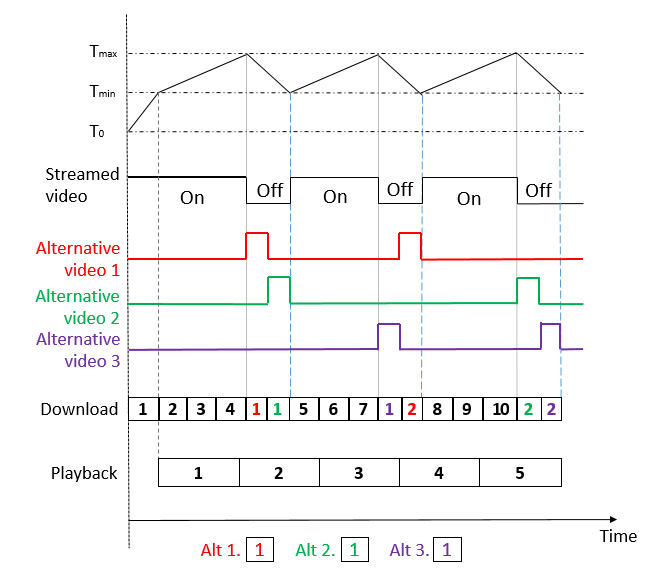
\includegraphics[scale=0.5]{prefetch.png}
	\caption{Prefetching overview}
	\label{fig:prefetch}
\end{center}
\end{figure}

\begin{figure}[t!]
\begin{center}
	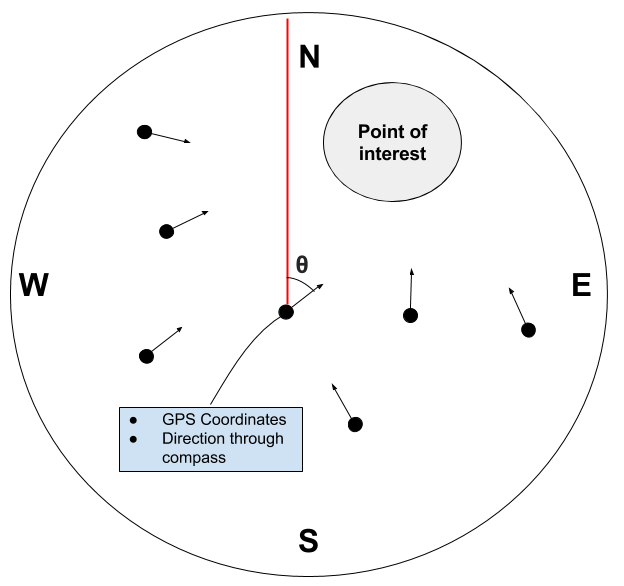
\includegraphics[scale=0.5]{teomet.png}
	\caption{Concept interface of GPS and Direction selection map}
	\label{fig:gpsinterface}
\end{center}
\end{figure}


The SMP player is by default set to play a stream of video located at a server supporting HTTP-streaming. For this project we'll be using the Adobe Media Server 5 for enabling the chunked video streaming needed for our HAS functionality. Since we will be using a similar OSMF player that were used in Krishnamoorthi et al. \cite{hasmultipath}, the quality of our prefetched chunks will be adaptive to the available bandwidth. \cite{hasmultipath}.

\begin{figure}[t!]
\begin{center}
	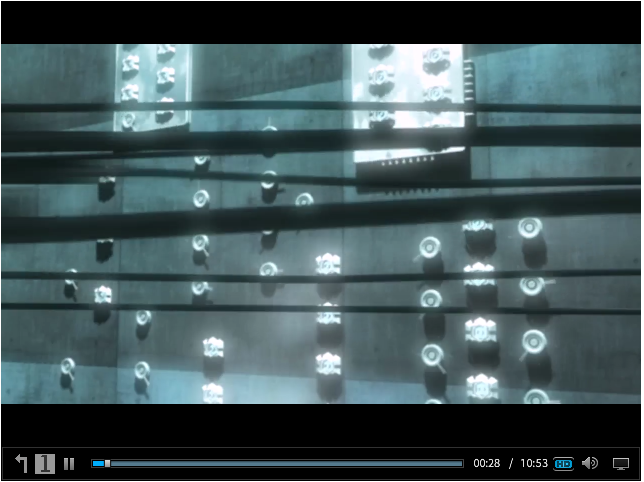
\includegraphics[scale=0.5]{Media_player.png}
	\caption{Strobe Media Player}
	\label{fig:mediaplayer}
\end{center}
\end{figure}

\subsection{Relative placement of Geographical Points}
The interface accepts an arbitrary number of video streams coupled with a cardinal direction and GPS-coordinates, including latitude and longitude values. The graphical points representing these video streams with coordinates should then be placed and scaled relatively to each other on the interface's geographical map, as shown in Figure \ref{fig:gpsinterface}. To accomplish this automatic placement and scaling we developed an algorithm to calculate where the points should be drawn to keep their relative positions between each other, so the graphical points accurately represents the real life locations of the recordings.

\subsubsection{Geographical Position algorithm}
The way the algorithm works is that every streamer and point of interest is an object in a list. Every object starts with having it's position in the middle of the geographical map. What the algorithm basically does is that it goes through each and every object in the list and checks its coordinates relative to the other ones. This is done be checking the objects' actual real-life distance between each other by calculating the difference between the coordinates of each object to get a relative distance between them. This is effectively done by using Pythagoras theorem like this:

\begin{align*}
x &= (longitude2-longitude1)*40000  \\
 &\phantom{b=\,} *cos((latitude1+latitude2 * \pi/360)/360) \nonumber \\
y &= (latitude1-latitude2)*40000/360 \\
z &= \sqrt{x^2+y^2}
\end{align*}

The equations above show the equireqtangular approximation formula. It's a simple method of calculating the distance between two geographical points on the surface of a spherical area \cite[s.~5]{equi}. In the formula we approximate the earth's circumference as 40000 km. X and y are the difference between two objects' longitude and latitude values translated to x- and y-coordinates to fit our geographical map as it represents a view on a flat plane. If we had used latitude and longitude as plain x and y values instead the positions wouldn't have provided a good enough accuracy to the flat x-/y-plane because of the spherical nature of latitude and longitude coordinates. An alternative method of calculating the distance between two objects would have been the Haversine formula, which excels at accuracy along high distances \cite{haversine}. For smaller distances used however, as in our project, equireqtangular projection suffices.

With x,y and z can the relative "move distance" be calculated. This move distance is a fixed distance in which an object will move relative to another one in the geographical map, depending on the number of objects to be drawn.

\begin{align*}
\label{eq:2}
valueX = moveDistance*|\frac{x}{z}| \\
valueY = moveDistance*|\frac{y}{z}|
\end{align*}

ValueX and ValueY are the distance in which an object will move in x-axis and y-axis respectively and moveDistance is the constant value which represents how much an object should move, this is set as the radius of the geomap to help with scalability. The reason we take the absolute value of x/y divided by z is to check where an object should move. When we have our scaling value the algorithm will check how to move the object relative to real-life. This check is to see if the object in real-life is more to the west, north, south or east in-order to know the direction for moving the object in x-axis and y-axis on our flat plane.

For scalability of our algorithm the value of moveDistance will be changed accordingly to the number of objects to place. This is done by dividing the moveDistance to number of users. The reason for this is because every object will move relative to every object in the list thus the distance one object has to move will be moveDistance times the number of objects. Another reason for doing this scalability is to ensure that an object won't be placed outside the geomap, however if that would happen then there is another fail-safe algorithm which will check if an object is outside the map and adjust it accordingly.

\subsubsection{Limitations and Accuracy}
The geographical position algorithm places every object relatively good compared to reality but it is not perfect and there is room for improvements. The accuracy of the algorithm is generally good in most cases but sometimes the relativite placement can seem a bit off. However in this case the object is not placed in a completely wrong place, but the object's x- and/or y-coordinates is wrong relative to another object. This mostly happends if we have too many objects, one or two objects relativity will be off but not with a large margin. The reason can be because we convert the latitude and longitude to x- and y-coordinates, however this can not be the whole problem since relativity is generally good for a few objects (less than ten objects).

While testing, in some cases when the number of objects exceeds 10, a few objects are placed in relatively different way compared to when the objects are fewer than 10. We are not entirely sure why but since our algorithm uses very simple equations and ideas then accuracy may decrease for many values because of our way of scaling the distance to move. The scaling distance may get so small that when rounding up to an integer the value will be of bay a small margin. This is the case when the few objects are placed relatively wrong, even though it seems wrong the margin of error is not big. Every cases tested shows that the margin in which the placement seem off is by a very small position in x-axis and y-axis. This will be shown in \textit{Section 4}.

%For now the algorithm will also utilize a countermeasure, which is meant to improve the relativite location between the objects. This countermeasure is that the way x-coordinates and y-coordinates is calculated in another way.

\begin{align*}
x &= longitude1-longitude2  \\
y &= latitude1-latitude2 \\
\end{align*}

The equation above is simpler and doesn't translate spherical longitude and latitude coordinates to flat x- and y-coordinates which leaves room for improvement, but for many objects in a small area this isn't as big of an issue. When the number of objects are many then there isn't as much of an issue since every object will move so little compared to one another that how much they move in x- and y-axis isn't as important. 

\subsection{Technical details}
Här skriver vi vad vi gjort i koden för att få allt att fungera. Att vi använt Advertisement plugin för att få saker att funka, och att vi dragit om lite kablar så att advertisementplugin ska fungera med flera videos och att det ska kunna gå att pausa och byta tid i filmerna (vilket inte gick innan ty advertisementplugin är gjort för opausbara reklamer).

To be able to accomplish switching between videos and getting a functional UI there are a lot of technical details to be explained in-order to get a full understanding of how the code works. Since we used the code from Krishnamoorthi et al.\cite{qualbranch} there was first a lot to understand before we could start doing anything. The problems we had and complications we encountered will be explained in the discussion while the focus here will be on \textbf{our} code and implementations. 

Our progressing can be divided into different sections which will be explained in a general detail:

\begin{enumerate}
\item Making a button to open the view.

\item Making a view appear with point of interest and cardinal directions.

\item Making clickable geo-map objects appear.

\item Connecting each geo-map object to a video and be able to play it through a class called AdvertisementPluginInfo.

\item Making the geo-map videos interactable.

%\item (Attempting to make the geo-map switching seamless.)This will be added to result/discussion instead.

\item Adjustments and improvements of the code and implementation of a position algorithm. 
\end{enumerate}

The details of the code and implementation will not be explained line by line but will give more a general idea and overview of what was done.

The first step was to make an interactive button which we open our view with. For this we had to create three different assets for how the button should look like, which we designed ourselves in photoshop. The button is illustrated as three arrows with a dot at each end facing a general direction. This shows that a view is opened with objects similar to those. These buttons where then added to a SWC (ShockWave Component) file which stores the assets. The assets was then handed an assets id and name so they could be retrieved. A class for the button was created that was added to the control bar. The button extended \textit{ButtonWidget} where we could add the assets to a face which allowed us to switch between the different assets when changing face. 

The second step was to make a view appear that is represented as circle to better fit with how geo-map objects will be placed. For this a widget and sprite class was created. The geo-map widget class handles size of the clickable layout, creation of the geo-map view and handling of fullscreen. The geo-map view is placed in the middle of the stage for the player and when fullscreen is initiated everything will be scaled such that relativity is kept. In the geo-map sprite class the position algorithm, creation of every object and cardinal direction is handled.

In the third step we created a new class called \textit{GeoMapObject} which will hold all our functions of the streaming video is shown on the view. This class will have functions to add and get the position of the geo-map object, the latitude and longitude, direction, setting the URL to be connected with the object etc. The geo-map object which is created in geo-map sprite is added to a list. This list will handle all the geo-map objects on the view and is used for when clicking on an object. Together with a function in the geo-map object class it helps to show which object is clicked on and make sure that no more than one object is highlighted at the same time.

When getting to the fourth step the technicalities became a bit more complicated and here is when the servers are used and getting the videos to play was about to happen. The server will be explained more later and also the difficulties and problems that occurred. For this step each video in the geo-map objects needed to be played and therefore a class called   \textit{AdvertisementPluginInfo} which is a class used for playing videos in the beginning, middle or end of a video. In this project a modified function of playing the video in the middle was used and made it so that instead of waiting for the video to change the switch and loading of the video would happen directly when the object is clicked on. To get this to work the class needed to first stop the main video and signal that another video is playing. For this the main media player from the Strobe media playback needed to be fetched and sent in to the \textit{AdvertisementPluginInfo} class. This was solved by creating the geo-map button in the SMP class and then sending in an instance which was forwarded to the geo-map objects. This way the media container and media player that the SMP played mainly could be stopped and removed. When this was done the \textit{AdvertisementPluginInfo} class could change between the different videos as they were an advertisement, this meant that only playing the video was possible but not interacting with it.

Step five, which was about getting the interaction for the video to work, was the most difficult task of them all. Since the video was played as an advertisement some things needed to be changed. The main thing here is that the media that is still recognized is the main media from the Strobe Media Playback while the geo-map video was only an advertisement on top of it. What was then done is that the advertisement media was added to all the controls that was used. In other words , instead of playing, pausing, interacting with the scrub bar for the main video a check is done for the controls. What this check does is that it checks if an "advertisement" is played and if it is then the controls will be changed to be on the advertisements player.

In the last step adjustments and improvements was done to the code and also the inclusion of the position algorithm. Here the code was adjusted and improved to make it such that the implementations that was done wouldn't crash anything else. Here the \textit{PointOfInterest} class was implemented to better fit the algorithm. Since the algorithm uses a list of all geo-map objects there was need for \textit{PointOfInterest} to be an object that uses similar functions to the ones in the geo-map object class. 



\subsection{Server and video application}
%Här skriver vi hur vi praktiskt tillämpat adobe flash-servern och hur den hänger ihop med Apache-servern. Även hur spelaren och mediaservern bara accepterar .f4v-filer och att vi konverterat våra egna filmer till det formatet.

As said earlier the server used is the Adobe Media Server 5 (AMS 5), which is primary used for downloading videos from cache as similar to the works described in \textit{Section 2}. The AMS 5 is a server used for HTTP streaming which is needed in-order to use HAS. The AMS 5 uses something called an Apache server, specifically Apache 2.4, which enables a video to be called with HTTP. To stream videos with the AMS 5 there can be a need to allow the the flash player to stream a HTTP-video through the local media player\footnote{Global\:Security\:Settings\:panel: https://www.macromedia.com/support/documentation/en/\\flashplayer/help/settings$\_$manager04.html} otherwise there can occur an security error. Reason being that a call is made in the code to a plug-in which allows for sending and requesting a URL to be played.

Except for using the AMS 5 to play a video through HTTP the video also needs to be in format of F4V or FLV which are two different video file formats used for delivering videos over internet using Adobe Flash player. Every video that has been filmed has been converted to FLV with FFmpeg\footnote{FFmpeg: https://ffmpeg.org/} which is a free software project that produces libraries and programs for handling multimedia data. It contains a program which allows us for transcoding media files.


\section{Validated Result}
%Testfall:Vi ställer oss utomhus på ett område i campus (utanför korallen/blå havet?) och filmar på 3-4+ ställen med lagom stort avstånd mellan varandra, med varierande riktningar. Gärna att vi filmar på en och samma punkt där det rör sig folk, samtidigt med olika kameror så att vi ser samma sak från olika håll. Vi antecknar koordinater för varje punkt vi filmar och väderriktningen.När det är avklarat så antecknar vi i rapporten de koordinater vi använt (på något sätt, i text eller i någon bild) och markerar ut koordinaterna i både Google Maps och vår karta, vilket demonstrerar att den relativa utplaceringsalgoritmen fungerar. Sen visar vi i rapporten två bilder där Media Playern står på samma tidsförlopp och visar samma (gärna rörande föremål/person) från två olika håll, vilket demonstrerar att vi kan byta videoströmmar för att få se samma sak från två olika ställen.

%Vi kunde bara filma med två kamror samtidigt så vi har tre st set av filmer som körs samtidigt.

%Mätningar:Tid det tar att byta film och så?

%(Tänkte skriva i resultatdelen om hur placeringar ser ut och vart saker placeras samt nämna hur många object som algorithmen klarar av att placera ut på relativt bra sätt mm.)

To demonstrate our geo-based mediaplayer, we went out and did some recordings to test every functionality we’ve been working in the mediaplayer on during this project. We went to “Blåa havet” in front of Kårallen located at Linköping Universitet where some students were promoting an upcoming event with some activities. We found that this was a suitable point of interest to record from different angles for our testing case. As we only had two cameras available we made three sets of recordings consisting of two recordings each, with each set displaying the same scene from two different locations and angles at the same time. The desired outcome of this test was to be able to swap between the recordings to view the same object at one point in time from different angles.


\subsection{Position Algorithm}
To demonstrate the accuracy of our relative placement of geographical points in our interface, we noted the GPS-coordinates and angles at the used recording locations. We then input the coordinates into Google Maps as seen in Figure \ref{fig:googlemaps}, which we will here use as a reference to prove the accuracy of our placement algorithm. We then input the same latitude, longitude and angle values into our interface and the result is shown in Figure \ref{fig:testfallgeomap}.


\begin{figure}[ht!]
\begin{center}
	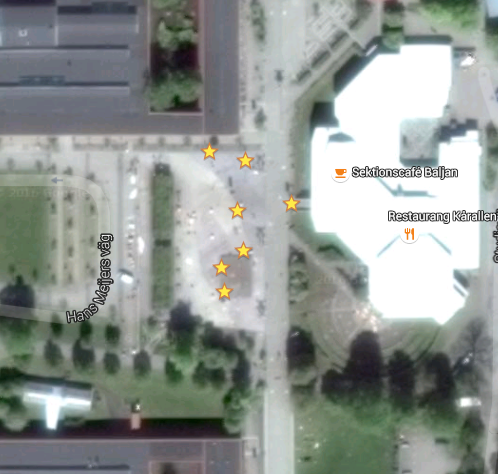
\includegraphics[scale=0.64]{Google_Maps.png}
	\caption{Google Maps view of the Streaming locations}
	\label{fig:googlemaps}
\end{center}
\end{figure}

\begin{figure}[ht!]
\begin{center}
	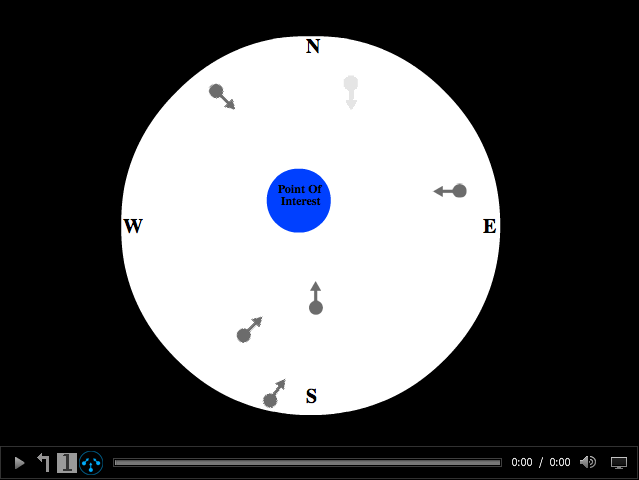
\includegraphics[scale=0.37]{TestfallGeomap.png}
	\caption{Geo-map view of the Streaming locations}
	\label{fig:testfallgeomap}
\end{center}
\end{figure}

The arrow-points in the geographic map is almost an exact match to those in the Google Maps screenshot, at least in terms in relativity. There is a slight difference between the two and the reason for this is that the points in our geographical map is scaled to make use the entire map, in such a way that the distance between them are increased while their relative locations between each other remain intact. This would prove the accuracy of our relative placement of the geographical points.


\subsection{Geo-based Streaming}
As we’ve mentioned before, our implementations is as shown in Figure \ref{fig:gpsinterface} where we have a button that opens the geographical map, a circle that represents a “map” and arrows pointing in a direction that represents streamers/videos. When a video is selected the arrow is highlighted and that video is then played. In our test case, we set up two cameras at a time and did recordings of 90 seconds each. In these videos we captured plenty of people doing plenty of stuff. There were people jumping the trampoline, using hoverboards, walking and biking around. When we input these 3 sets of two recordings each into our mediaplayer, we could swap between the two recordings and watch these same events unfold from different positions and angles. In Figure \ref{fig:testview1} and \ref{fig:testview2} two different recordings are selected and they show the same event where, for example, the guy inside the red circle in the pictures are hoverboarding in front of the red shirt guy the same time. This would prove the desired functionality of where the user can display the same event from different geographical positions and angles.

\begin{figure}[ht!]
\begin{center}
	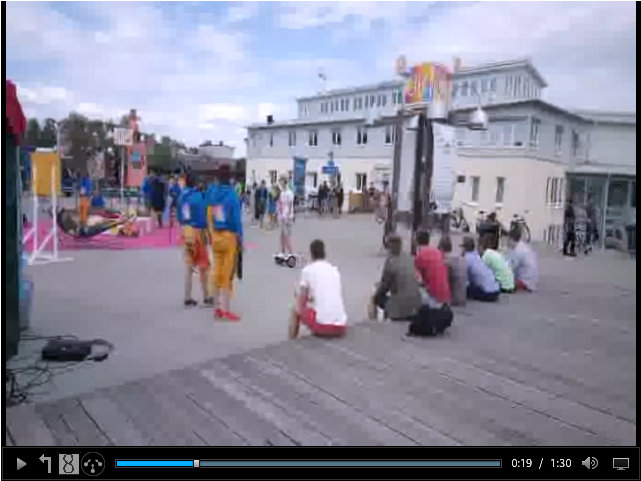
\includegraphics[scale=0.5]{Hoverboard_1.png}
	\caption{Test view 1}
	\label{fig:testview1}
\end{center}
\end{figure}

\begin{figure}[ht!]
\begin{center}
	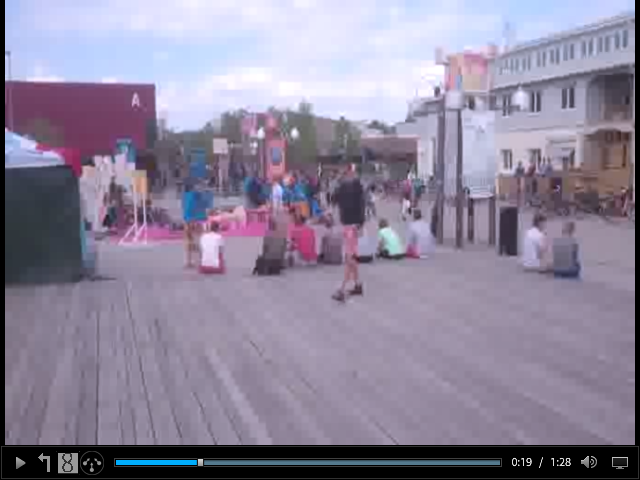
\includegraphics[scale=0.5]{Hoverboard_2.png}
	\caption{Test view 2}
	\label{fig:testview2}
\end{center}
\end{figure}



\section{Discussion}
When we started working on this assignment to make an interactive Command-and-Control center with geo-tagged streaming we first had to install and adjust to the tools given to us to develop the interface, being OSMF and SMPl. These tools consisted of an extensive amount of existing code which we had to delve into and understand for us to implement our features.
This was a process which took some time since we also weren’t very familiar with the language enviroment, Adobe ActionScript 3.0. ActionScript is an object-oriented programming language developed by Adobe Systems and influenced by JavaScript, while its syntax still being relatively similar to Java which we had previous experience with. Eventually we got a better understanding on how to operate in this new enviroment and reverse engineer the provided code. However there were still many sections of the code which we didn’t understand or knew that we would need in our work, and wrapping our heads around this took more time than we would have wished. 

At the start of this project we focused much of our time to understand the principles of HAS, geographical based streaming, prefetching and how to implement them into our own interface. While we did have a good grasp on how these principles works and had a good idea of how we would go around to implement them, we couldn’t quite get it to work. Since we used code from a previous work we made the assumption that as long as our implementation of our interface’s features was similar to that previous work, the HAS would function. Flash builder, SMP and the HAS-functionality in the provided code required the video files to be split into the formats F4M, F4X and F4F when doing the prefetching. We were also provided with some video test files from our supervisor which he used when he worked on the HAS-functionality in his code. This didn’t work since some codebits didn’t run properly. There are two things that may be the cause of this. The first thing is that we didn’t do what was neccessary to get it to work because our lack of understanding of how the HAS-functionality actually operates in the code and how we would need to rewrite the existing code to function with swapping between several videos. It didn’t work out of the box because it HAS in the provided was hard coded to only support one video and our attempts at supporting multiple video streams ended in failure even with the help of the HAS-functionality code’s author himself. The second cause of this might be because the changes we did to the provided code in our implementation weren’t correct. If we were to look at those two cases the first one seems to be the more plausible one, since we assumed that the code we got would just work as long as we had the assets and did a similar implementation to the one our supervisor had done. The second one seem less likely since the changes we made to the code was so that it wouldn’t disrupt the HAS or media player in anyway, however it could also be a possibility. 

Because we couldn’t get the HAS-functionality to work properly we therefore couldn’t get the prefetching of different video streams to work. Our focus and time throughout most of the project was very much put on the prefetching, but since we couldn’t get it to work we switched our focus to a better implemented and function command-and control interface.
This included improving the interface to work properly whether the player was in standard or fullscreen mode, each geographical map object displaying GPS-coordinates and direction of the video stream while hovering over it and the relative position placement algorithm for drawing the objects. The position algorithm took some time to implement but we had initially a general idea of how it should work. When we developed it we worked on two similar but separate solutions each to see which one worked best, but since it took more time than expected only one solution was finished in time which proved feasible and then used. The main challenge with developing this algorithm was to provide relativity, scalability and accuracy up to our standards which caused the algorithm to take some time to create.

When developing the position algorithm we looked at several ways to translate the spherical longitude and latitude to accurate grid x- and y-coordinates. In the end the decision was between the two formulas haversine and equirectangular approximation. The formula that was used in the end was equirectangular projection because that’s the first one we tried to implement with the algorithm and worked well. Since the accuracy of equirectangular approximation apparently is slightly worse than that of the haversine formula, we could have compared the use of both formulas to see if there were any significant difference in the implementation between the two \cite{haversine}. Nonetheless the final algorithm is up to the standard that we envisioned. 

For our test case, there is one thing we in hindsight would have changed if we would have redone it. In our case we set up only two cameras at a time to get multiple views of what was happening at the scene from different locations, simultaneously. To further and better prove the functionality of our user interface in a test case, we should have brought some more volunteers and cameras along with us to get even more point of views of the same scene at one point in time. While doing two recordings at once was enough to prove the functionality of this feature, more recordings would have been a neat addition. 

Furthermore as mentioned previously in this report, Adobe Flash is becoming more deprecated by the day even by Adobe themselves. Because of this, if the project was redone the interface would be better suited to be implemented in the mediaplayer built from a more modern alternative such as Flash’s main competitor, or rather replacement, HTML5.

One big obstacle which cost a lot of unneccary time was the setting up of the used server. We initially we used something called a WAMP server at the start of the project which enabled us to stream videos using HTTP through an Apache HTTP Server. However, since idea of prefetching was still present at that point of the project there was a need to switch to Adobe Media Server 5 since it would allow us to stream chunked bits of video used for the prefetching. While setting up the servers we ran across numerous problems with different kinds of security errors which wouldn’t allow us to stream the videos using HTTP. While trying to solve these issues we found that since the Apache server ran on a Windows 10 client there was a process that blocked the server that was needed to be stopped. Only then was the server able to run and allow videos to be streamed with HTTP.

If the project was redone we would have made a more definite time plan of what was needed to be done. Our time plan, even though straigthforward, wasn’t very detailed. We knew what we wanted to accomplish and when but we didn’t really know how we would go about to accomplish it. This ended up unnecessarily consuming a lot of time since we didn’t know where to look in the giant web of provided code to solve any eventual issues or where exactly to implement the changes and solutions.

\section{Conclusion}

This project provides a command-and-control center UI which allows for video streams to be changed on-demand with the use of an interactive geographical position map with video stream locations tagged with GPS-coordinates including latitude and longitude values and cardinal directions, implemented in Strobe Media Playback. The interactive map provides details of where streamers are positioned relative to each other. This is handled through an algorithm that places every object on the map relative to how the objects, representing the recordings, in the real world are located. The accuracy of the algorithm is shown to be placing each object relatively good to one another with a good accurracy, at least when the number of objects doesn’t exceed ten. By creating an object with a latitude, longitude and direction it will show this information of the object while hovering over it. Besides the locations of the streams there is also a point of interest drawn in the map which is also using this algorithm. Each stream is clickable and displays its representative video in the mediaplayer when clicked. The object representing the current recording playing will then be highlighted when the geographical map is reopened to show that this video is currently loaded and played. All the videos are interactable and when switching videos the point of time in the recording will be transferred to the next video in order to allow for the user to see the same situation and swap between different locations and angles. Even though seamless, uninterrupted switching through prefetching was not achieved because of several difficulties the code provided is made in a way that prefetching should be easy to implement with our developed interface. The features of this interface should allow for a good way for people to stream and interact with videos during a concert or disaster event in way that will make experience and work easier to accomplish. For future work, when prefetching is added, the switching between different videos will be seamless and further improve the quality of service of the geo-based mediaplayer.

\section{Acknowledgement}
During this project we want acknowledge...

\clearpage
\begin{thebibliography}{9}

\bibitem{gtube}
  Jia Hao, Roger Zimmermann, Haiyang Ma,
  \emph{GTube: Geo-Predictive Video Streaming over HTTP in Mobile Environments}.
  \newline
  Published: 2014. Fetched: 2016-03-09 
  \newline
	URL: \text{http://goo.gl/6DiQiW}.

\bibitem{qualbranch}
  Vengatanathan Krishnamoorthi, Niklas Carlsson, Derek Eager, Anirban 
Mahanti, and Nahid Shahmehri,
  \emph{Quality-adaptive Prefetching for Interactive 
Branched Video using HTTP-based Adaptive Streaming}.
  \newline
  Proc. ACM 
International Conference on Multimedia (ACM Multimedia), Orlando, FL, Nov. 2014, pp. 317--326.

\bibitem{osmf}
  Greg Hamer,
  \emph{Open Source Media Framework: Introduction and overview}.
  \newline
  Published: 2010-03-15. Fetched: 2016-03-09
 \newline
  URL: http://www.wi-fiplanet.com/tutorials/article.php/3433451/Implementing-Wi-Fi-Multicast-Solutions.htm.
  
  \bibitem{streamrate}
  T. Huang, N. Handigol, B. Heller, N. McKeown, and R. Johari,
  \emph{Confused, timid, and unstable: Picking a video streaming rate is hard.}.
  \newline
  In Proc. ACM IMC (November 2012).
  
  \bibitem{hasmultipath}
  Vengatanathan Krishnamoorthi, Patrik Bergström, Niklas Carlsson, Derek 
Eager, Anirban Mahanti, and Nahid Shahmehri,
  \emph{Empowering the Creative User: 
Personalized HTTP-based Adaptive Streaming of Multi-path Nonlinear Video}.
  \newline
  Proc. ACM 
Proc. ACM SIGCOMM Workshop on Future Human-Centric Multimedia Networking 
(FhMN), Hong Kong, Aug. 2013, pp. 53--58.

\bibitem{bandawarePrefetch}
Vengatanathan Krishnamoorthi, Niklas Carlsson, Derek Eager, Anirban 
Mahanti, and Nahid Shahmehri,
	\emph{Bandwidth-aware Prefetching for Proactive 
Multi-video Preloading and Improved HAS Performance}.
	\newline
	Proc. ACM 
International Conference on Multimedia (ACM Multimedia), Brisbane, 
Australia, Oct. 2015.

\bibitem{scalableOnDemand}
Zhao, Y., D. L. Eager, and M. K. Vernon,
	\emph{Scalable On-Demand Streaming of 
Nonlinear Media}
	\newline
	 IEEE/ACM Trans. on Networking, Vol. 15, No. 5 (Oct. 
2007), pp. 1149-1162.

\bibitem{bufferbased}
T. Huang, R. Johari, and N. McKeown,
	\emph{ Downton abbey without the hiccups: Buffer-based rate adaptation for HTTP video streaming.}
	\newline
	 In Proc. ACM SIGCOMM FhMN
Workshop, Aug. 2013.

\bibitem{equi}
John P. Snyder
	\emph{Flattening the Earth: Two Thousand Years of Map Projections}
	\newline
	University Of Chicago Press, 1993
	
\bibitem{haversine}
Doctor Rick,
	\emph{Deriving the haversine formula}.
	\newline
	Published: 1999-04-20. Fetched: 2016-04-11.
	\newline
	URL: \text{http://mathforum.org/library/drmath/view/51879.html}


%\bibitem{randall2008}
%	Randall D. Knight,
%	\emph{Physics for Scientists and Engineers: A %Strategic Approach with Modern Physics (2nd %Edition)}.
%	\newline
%Addison-Wesley, 2a upplagan, 2008.

%\bibitem{polesAndZeros}

%	\emph{Understand Poles and Zeros}.
%	\newline
%	Publicerad 2002-11-01. Hämtat: 2015-06-01.
%	\newline
%	URL: http://web.mit.edu/2.14/www/Handouts/PoleZero.pdf

\end{thebibliography}

%%removes page number from this page
\thispagestyle{empty}

\end{document}
